%%%%%%%%%%%%%%%%%%%%
%
% $Beschreibung: Schrittmotorbeschreibung allgemein und speziell für den NEMA 17 $
% $Autor: Stein und Theilmann $
% $Datum: 05.04.2024 $
% $Pfad: DemonstratorSchrittmotor/DeveloperDoc/Contents/de/Schrittmotorbeschreibung.tex $
% $Version: 1 $
%
%
%%%%%%%%%%%%%%%%%%%

\chapter{Schrittmotor}

In diesem Kapitel folgt eine grundsätzliche Beschreibung eines Schrittmotors. Darauf folgt die Erläuterungen zum Aufbau und Funktionsweise eines Schrittmotors sowie die Aufzählung verschiedener Grundbauarten.

\section{Beschreibung eines Schrittmotors}

Ein Schrittmotor ist ein Elektromotor, der sich für präzise Positionierungsaufgaben eignet. Im Gegenteil zu anderen Elektromotoren wird bei einem Schrittmotor keine Positionsmessung oder Positionsregelung benötigt. Andere mechanische Antriebssysteme benötigen einen geschlossenen Regelkreis und mechanische Bremsen um Drehzahl und Position einzuhalten. Der Motor führt durch die Rotation des Rotors diskrete Schritte aus, wobei jeder Steuerimpuls eine Verschiebung um einen konstanten Winkel bewirkt. Mit diesem Motor ist eine erreichbare Positioniergenauigkeit von 0,1° möglich. Diese Art von Elektromotor wird beispielsweise in Druckern oder Scanner, aber auch im Kraftfahrzeugbereich verwendet. Im Kraftfahrzeugbereich werden die Schrittmotoren zur Spiegelverstellung sowie der Sitzverstellung verwendet. Das maximal erreichbare Drehmoment eines Schrittmotors liegt bei zwei Newtonmeter und die maximal erreichbare Drehzahl bei ca. 2000 Umdrehung pro Minute. Der Vorteil eines Schrittmotors ist die Wartungsfreiheit, da der Rotor keine Wicklungen hat. \cite{Babiel.2023}\cite{Hagl.2021}\cite{Bernstein.2018}\cite{Schroder.2021}

\subsection{Aufbau und Funktionsweise eines Schrittmotors}

Der Schrittmotor besteht aus einem Stator, einem Rotor ohne Wicklungen und einer Steuerelektronik. Diese Steuerelektronik setzt sich zusammen aus einer Treiberstufe und der eigentlichen Steuerung. Bei dem Stator handelt es sich um den feststehenden äußeren Teil und bei dem Rotor um den beweglichen inneren Teil, wie in Abbildung \ref{HaPrSchritt} zu erkennbar ist. Im Stator sind Spulen verbaut, die von einem Strom durchflossen werden. Hierdurch entsteht ein magnetisches Feld. Da der Rotor magnetisch ist, folgt er dem Magnetfeld des Stators. Soll eine Bewegung hervorgerufen werden, werden einzelne Wicklungsstränge ein- aus- oder umgeschaltet. Durch diesen Vorgang wird ein rotierendes Magnetfeld erzeugt. Das erzeugte Magnetfeld zieht den Rotor an. Der Rotor wird bei jedem Puls (Takt) um einen Winkelschritt weitergeschaltet. Die Anzahl der Polpaare im Stator geben die Anzahl der Schritte vor. Die Drehzahl und die Drehrichtung hängt von der Reihenfolge und der Häufigkeit der Stromimpulse ab. Es gibt drei verschiedene Betriebsarten, die abhängig von der Genauigkeit und der Drehzahl sind. Im Vollschrittbetrieb werden alle Polpaare bestromt. In dem Halbschrittbetrieb wird die Schrittzahl des Motors verdoppelt, wodurch sich die Positionsauflösung im Gegensatz zum Vollschrittbetrieb verdoppelt. Allerdings wird in diesem Betrieb das Drehmoment reduziert. In dem Mikroschrittbetrieb bewegt sich der Rotor in sehr kleinen Schritten. Hierdurch wird eine hohe Positioniergenauigkeit und ein ruhiger Lauf erreicht, da die Ströme und das Drehmoment in kleineren Schritten verändert werden. Bei einer zu hohen Schrittfrequenz kann ein Schrittverlust entstehen. Bei einem Schrittverlust überspringt der Motor einzelne Winkelschritte und landet in einer vorherigen oder nächsten Position gleicher Phase. Durch die offene Steuerkette werden die Verluste nicht erkannt.    \cite{Hagl.2021}\cite{Bernstein.2018}\cite{Schroder.2021}

\subsection{Schrittmotor Bauformen}

Wie bei anderen Elektromotoren gibt es auch bei dem Schrittmotor verschiedene Grundbauarten. 

\begin{itemize}
	\item {Permanentmagneterreger-Schrittmotor (PM-Schrittmotor)}
	\item {Reluktanzschrittmotor (VR-Schrittmotor)}
	\item {Hybridschrittmotor (HY-Schrittmotor)}
\end{itemize}

Der \textbf{permanentmagnetische Schrittmotor} hat einen Permanentmagneten in dem Rotor verbaut. Hierbei stellt sich der permanentmagnetische Rotor immer so, dass der Nordpol des Rotors dem Nordpol des Statorfeldes gegenüber liegt und der Südpol des Rotors dem Südpol des Statorfeldes. In dieser Ausrichtung ziehen sich die Pole gegenseitig an. Die Drehrichtung des Rotors hängt von der Fließrichtung des Stromes ab. Der permanentmagnetische Schrittmotor entwickelt im ausgeschalteten Zustand ein Drehmoment zur Selbsthaltung. Dies ist aufgrund des permanentmagentischen Rotors möglich. Bei diesem Drehmoment handelt es sich um das höchste Drehmoment, das auf die Welle des Motors übertragen werden kann, ohne dass diese sich in eine rotierende Bewegung versetzt. Zu dieser Art von Schrittmotoren gehören beispielsweise der Klauenpol-Schrittmotor und der Scheibenmagnet-Schrittmotor. Bei der zweiten Bauart handelt es sich um den \textbf{Reluktanzschrittmotor}. Bei dieser Bauart besteht der Rotor aus einem weichmagentischen Material und besitzt eine gezahnte Form. So lange der Schrittmotor von keinem Strom durchflossen wird, entsteht kein Magnetfeld. Sobald der Motor in Betrieb genommen wird, entsteht ein magnetischer Fluss innerhalb des Rotors. Wird nun eine Wicklung erregt, wird der nächste Zahn des Rotors angezogen. Dadurch, dass die Rotorzähne ungleich der Polteilung sind, kann das System unendlich lange fortgesetzt werden. Die Anzahl der Schritte und die Genauigkeit des Reluktanzschrittmotors ist abhängig von der Anzahl der Zähne auf dem Rotor. Aus technischer Sicht sind mit dieser Bauart Schrittwinkel unter 1° möglich. Damit die Drehrichtung verändert werden kann, sind mindestens zwei Strangwicklungen nötig. Bei den \textbf{Hybridschrittmotoren}, auch bekannt als HY-Schrittmotoren handelt es sich um eine Kombination aus dem Reluktanzschrittmotor und dem Permanentmagneterreger-Schrittmotor. Durch diese Kombination aus den beiden Schrittmotoren werden die Vorteile aus der kleinen Schrittweite, dem hohen Drehmoment und dem Selbsthaltemoment genutzt. Bei dem HY-Schrittmotor besteht der Rotor aus zwei um eine halbe Zahnteilung versetzten weichmagnetischen Polrädern, die eine zahnförmige Form haben. Bei den beiden Polrädern bildet das eine Polrad den Nordpol und das zweite Polrad den Südpol. Zwischen den beiden Polrädern befindet sich ein Permanentmagnet. Anders als bei anderen Schrittmotoren wird der Rotor bei dieser Bauart axial magnetisiert. Damit ein kleiner Schrittwinkel möglich ist, haben die Statorpole ebenfalls eine zahnförmige Form. Die Ausrichtung des Rotors ist abhängig von der Stromrichtung und wird durch den minimalen Widerstand bestimmt, der sich aus dem Stromfluss durch die einzelnen Stränge ergibt. Wird ein besonders kleiner Schrittwinkel benötigt, kann dies durch Erhöhung der Zähnezahl erreicht werden. \cite{Schroder.2021} \cite{Hagl.2021} \cite{Babiel.2023}

\subsection{Betriebsarten unipolar und bipolar}

Neben den oben bereits genannten Betriebsarten, kann außerdem zwischen dem Unipolarbetrieb und dem Bipolarbetrieb unterschieden werden. Der große Unterschied zwischen den beiden Betreibsarten besteht darin, dass in dem Unipolarbetrieb der Strom in eine Richtung fließt. Bei dem Bipolarbetrieb hingegen fließt der Strom in beide Richtungen. Dies ist möglich, da jeder Wicklungsstrang über eine Vollbrücke gespeist wird. Ein weiterer Unterschied besteht in der Schaltung der Zweige, durch die ein Gleichstrom fließt. In dem Unipolarbetrieb werden die beiden Zweige in Reihe geschaltet. Jeder Wicklungsstrang wird mit zwei Drähten parallel gewickelt. Sind die beiden Wicklungsstränge in dem Bipolarbetrieb parallel gewickelt, müssen die Zweige parallelgeschaltet werden. Im Bipolarbetrieb kann ein höherer Wirkungsgrad erzielt werden, wo hingegen der Unipolarbetrieb eine deutlich einfachere Schaltung aufweist. \cite{Schroder.2021}

\section{Beschreibung des verwendeten Schrittmotors}

Für das Automatisierungsprojekt wird ein Nema 17 Schrittmotor der Firma Creality3D verwendet. Dieser Schrittmotor wird im 3D-Druck sowie in CNC-Maschinen eingesetzt. Der Motor arbeitet im Bipolarbetrieb und es sind zwei Spulen verbaut. Er hat einen Schrittwinkel von 1,8 ° und benötigt somit 200 Schritte für eine volle Umdrehung. Die Wellenlänge beträgt 20 mm und der Wellendurchmesser 5 mm. Der ausgewählte Schrittmotor arbeitet mit einer Nennspannung von 12 Volt. Dadurch, dass er mit einer niedrigen Spannung arbeitet, kann kein hohes Drehmoment erzeugt werden. Dies wird qualitativ in der Abbildung \ref{DrehmomentDiagramm} für den Schrittmotor GM42BYG015 dargestellt. Hier ist zu erkennen, dass der Schrittmotor ein Drehmoment von ca. 0,8 kg$\cdot$cm erreicht. Auf der x-Achse wird die Geschwindigkeit in Pulses per Second (PPS) angegeben, d.h. die Anzahl der Steuerimpulse pro Sekunde. Der Schrittmotor erzielt aber eine gute Positioniergenauigkeit durch den kleinen Schrittwinkel und die Microstepp-Funktion. Des weiteren arbeitet der Motor mit 0,84 Amper pro Phase. Weitere Vorteile des Schrittmotors sind die kompakte Bauform mit den Abmessung 42 x 42 x 34 mm sowie die geringe Masse mit 220 Gramm. Betrieben werden kann der Schrittmotor in einer Umgebungstemperatur von -10\ °C bis +50\ °C.\cite{Gems.2024}

\begin{figure}[H]
	\centering
	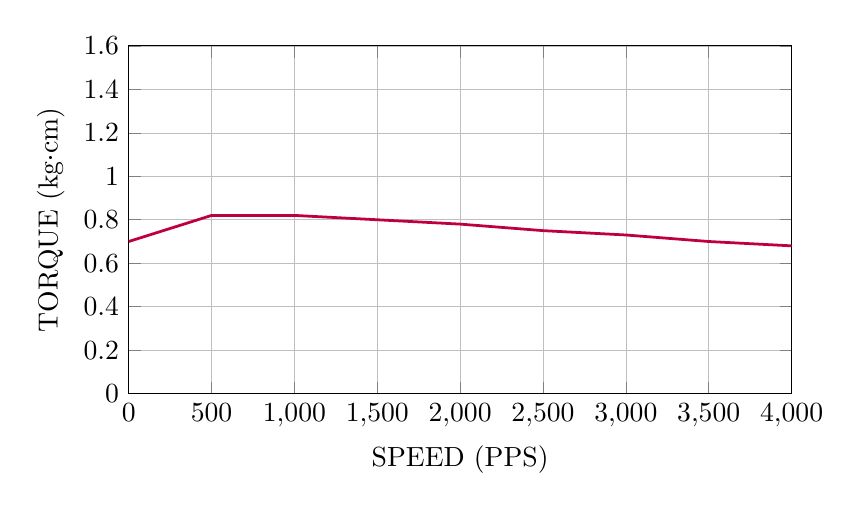
\begin{tikzpicture}
		\begin{axis}[
			width=10cm,
			height=6cm,
			xlabel={SPEED (PPS)},
			ylabel={TORQUE (kg·cm)},
			xmin=0, xmax=4000,
			ymin=0, ymax=1.6,
			xtick={0,500,1000,1500,2000,2500,3000,3500,4000},
			ytick={0,0.2,0.4,0.6,0.8,1,1.2,1.4,1.6},
			legend pos=north east,
			grid=both,
			major grid style={line width=.2pt,draw=gray!50},
			minor grid style={line width=.1pt,draw=gray!20},
			]
			\addplot[
			color=purple,
			line width=1pt
			]
			coordinates {
				(0,0.7)
				(500,0.82)
				(1000,0.82)
				(1500,0.8)
				(2000,0.78)
				(2500,0.75)
				(3000,0.73)
				(3500,0.7)
				(4000,0.68)
			};
		\end{axis}
	\end{tikzpicture}
	\caption{Drehmoment-Diagramm für den Schrittmotor 42BYG015}
	\label{DrehmomentDiagramm}
\end{figure}